\newpage
\section{Evaluation}
\label{sec:eval}
%
\begin{figure}[b]
\centering
\begin{center}
\begin{scriptsize}
\begin{tabular}{|l |  l | l|} 
\hline
 \multicolumn{1}{|c}  {\bf Benchmark} & \multicolumn{1}{c} {\bf
 Consistency} & \multicolumn{1}{c|}  {\bf
 Description}\\ [0.5ex] 
\hline
Counter  & MR & {Monotonicly increasing counter, e.g.
YouTubes' watch 
count}\\ \hline
DynamoDB  & RMW & {Integer register allowing various conditional puts and gets} \\ \hline
Online Store & RMW &  {Online store with shopping carts
and modifiable item prices} \\ \hline
Bankaccount  & 2VIS $\wedge$ RMW & {Offering deposit, withdraw and get balance operations}\\ \hline
Shopping List   &  MW $\wedge$ RMW & {A shopping list with
concurrent adds and deletes functionality}\\ \hline 
Microblog  &  MW, RMW & {A Twitter-like application modeled after
Twissandra}\\\hline
Rubis  & RMW, RMW$\wedge$2VIS & {eBay-like
application with browsing, supporting user wallet} \\
\hline
\end{tabular}
\end{scriptsize}
\end{center}
\caption{Fine-grained consistency requirement in benchmark programs}
\label{fig:dist_table}
\end{figure}

%intro: benchmark programs
%%%SJ: you need to introduce the implementation - what is
%%%the implementation written in, what does it run on top of,
%%%experimental setup, etc.
In this section, we present an evaluation study of our implementation,
including a report on
benchmark applications that utilize fine-grained weak consistency
requirements, expressable
in \tool's specification language.
Fig.\ref{fig:dist_table} presents seven such programs, that include
library definitions of individual replicated data types as well as
larger applications consisting of multiple replicated types. 

%multiple consistency levels for each program
%%%SJ: This is a very confusing paragraph - what is CC, what does
%%%length 1 or 2 mean in this context?
Each program supports various operations, some of which have
non-trivial consistency requirements. Out of the 38 non-SC operations
defined in these programs, there are 11 such operations, whose
consistency requirements can be expressed as a combination of four
previously described consistency guarantees: Monotonic Reads (MR),
Monotonic Writes (MW), Read-My-Writes (RMW), and Transitive Vis
(2VIS). The significant diversity among the consistency requirements
of these operations emphasizes the need for a multi-abled environment
that can understand and enforce fine-grained consistency requirements
efficiently. It is clearly not practical to hard code them all, due
their sheer number; even if we ignore bespoke consistency
requirements, there are 15 combinations of just the 4 aforementioned
consistency guarantees, even as there are other known guarantees, such
as writes-follow-reads (WFR), which we ignored.  Causal Consistency
(CC), the strongest of the weak consistency guarantees, is often used
as a metaphorical one-size to fit all weak consistency requirements.
Notably, none of the operations we analyzed intrinsically require CC.
Furthermore, we found that enforcing CC is significantly more
expensive than enforcing weaker guarantees (see below), thus making CC
a bad substitute for weaker guarantees. One the other hand, we found
\tool's generic consistency enforcement mechanism to be very useful in
this case.

%
%example
While the consistency requirements of the applications in
Fig.~\ref{fig:dist_table} are expressible as the combination of known
guarantees as described above, this is not necessary in general. The
bespoke consistency specifications of an application are usually
crafted by analyzing the anomalies that need to be prempted.  For
example, consider a bank account application, which offers \dRV{},
\wdRV{} and \gbRV{} operations, where \wdRV{} is a strongly consistent
operation that succeeds only if there are sufficient funds in the
account. There are two anomalous scenarios associated with \gbRV{} in
this program: \begin{enumerate*}[label=(\roman*)] \item when a user
      performs a \dRV{} that is not reflected in subsequent \gbRV{}
    operations; \item when a \gbRV{} witnesses a \wdRV{} effect
without witnessing all \dRV{} effects visible to it,  resulting in
\gbRV{} returning a potentially (incorrect) negative balance.
\end{enumerate*} The consistency specifications of  the bank account
application are crafted to preempt these anomalies. As presented in
Fig.~\ref{fig:dist_table}, \gbRV{} requires both \rmwCTRT{} and
\visCTRT{} guarantees to be simultaneously satisfied.
\begin{figure}[t]
        \centering
	\begin{subfigure}[t]{0.25\textwidth}
	\centering
	\hspace{-13mm}
	
\includegraphics[scale=0.22]{Figures/latency.pdf}
	\subcaption*{ \hspace{-10mm} (a) Latency}
	\end{subfigure}
	\begin{subfigure}[t]{0.36\textwidth}
	\centering
	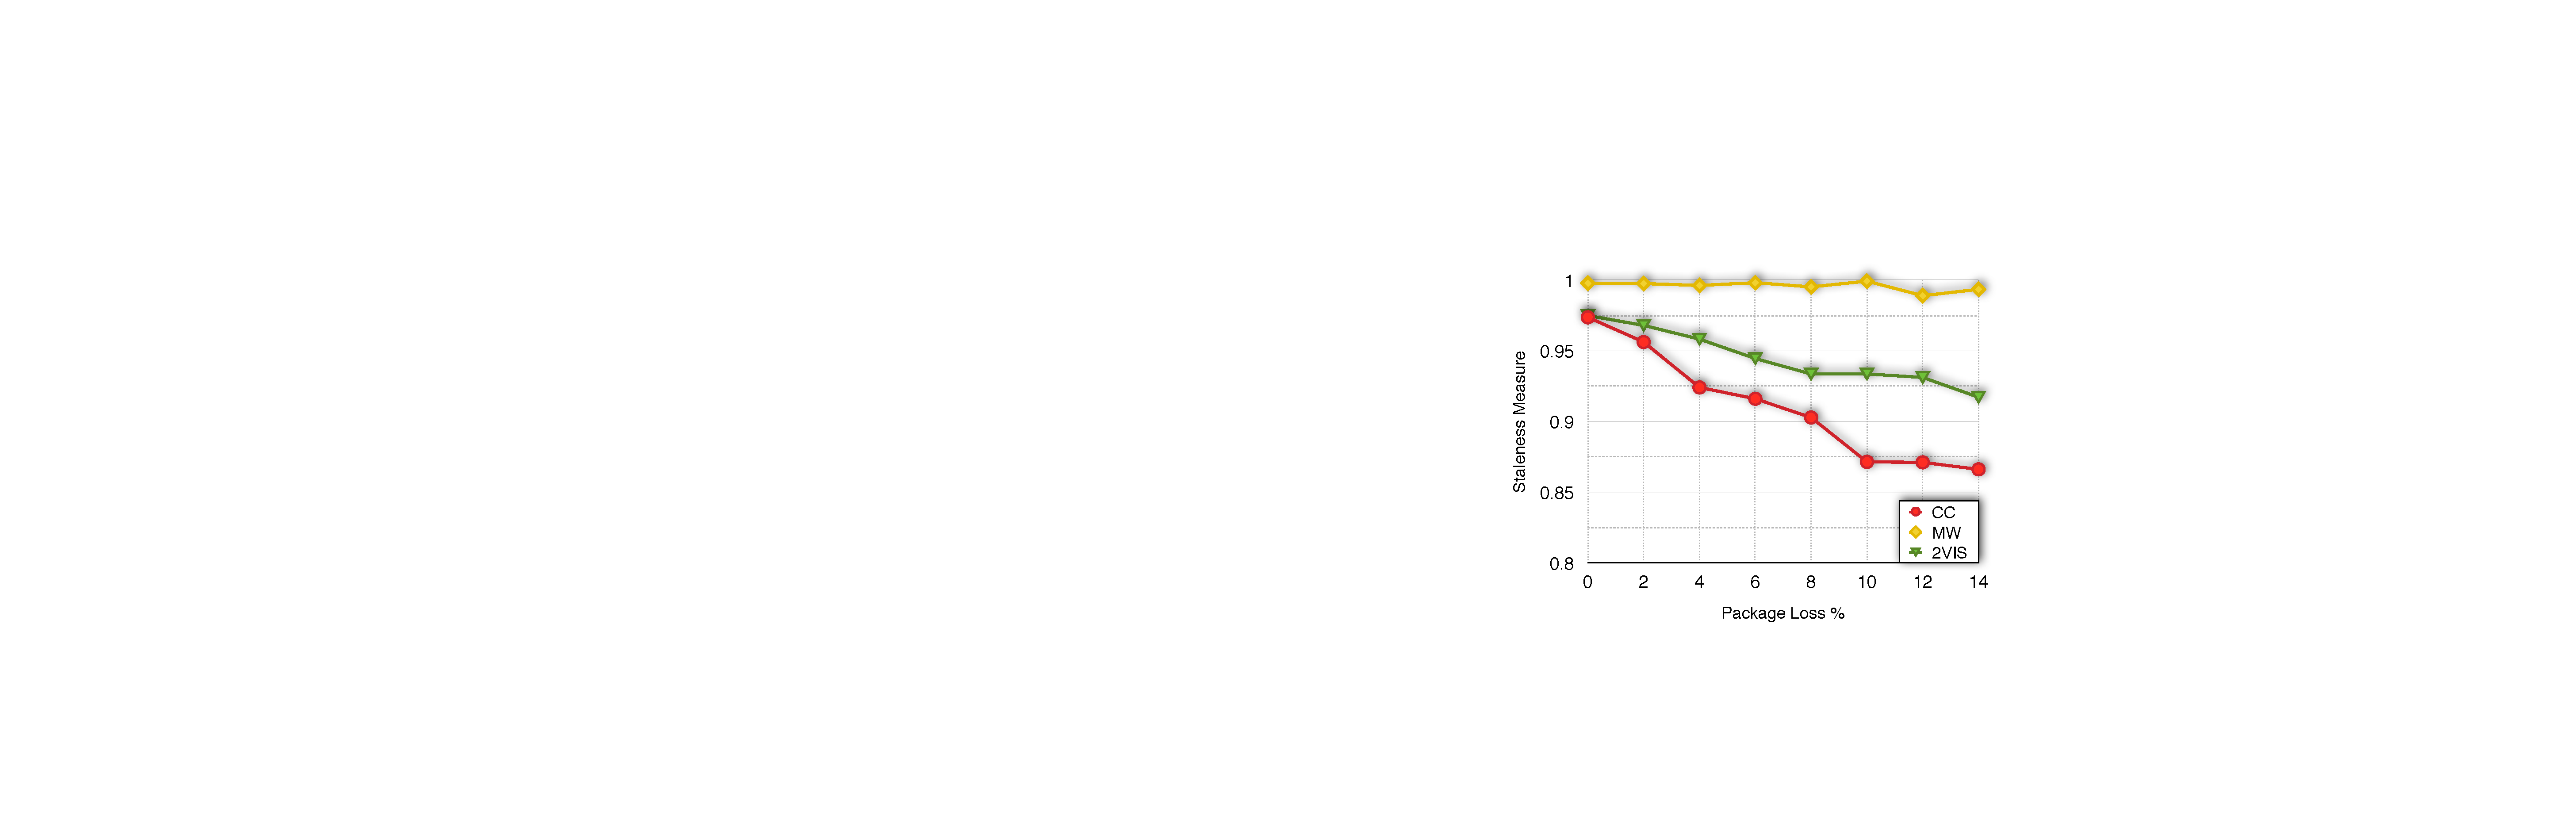
\includegraphics[scale=0.22]{Figures/staleness.pdf}
	\subcaption*{ \hspace{-1mm} (b) Staleness}
	\label{subfig:comment_example}
	\end{subfigure} 
	\begin{subfigure}[t]{0.28\textwidth}
	\centering
	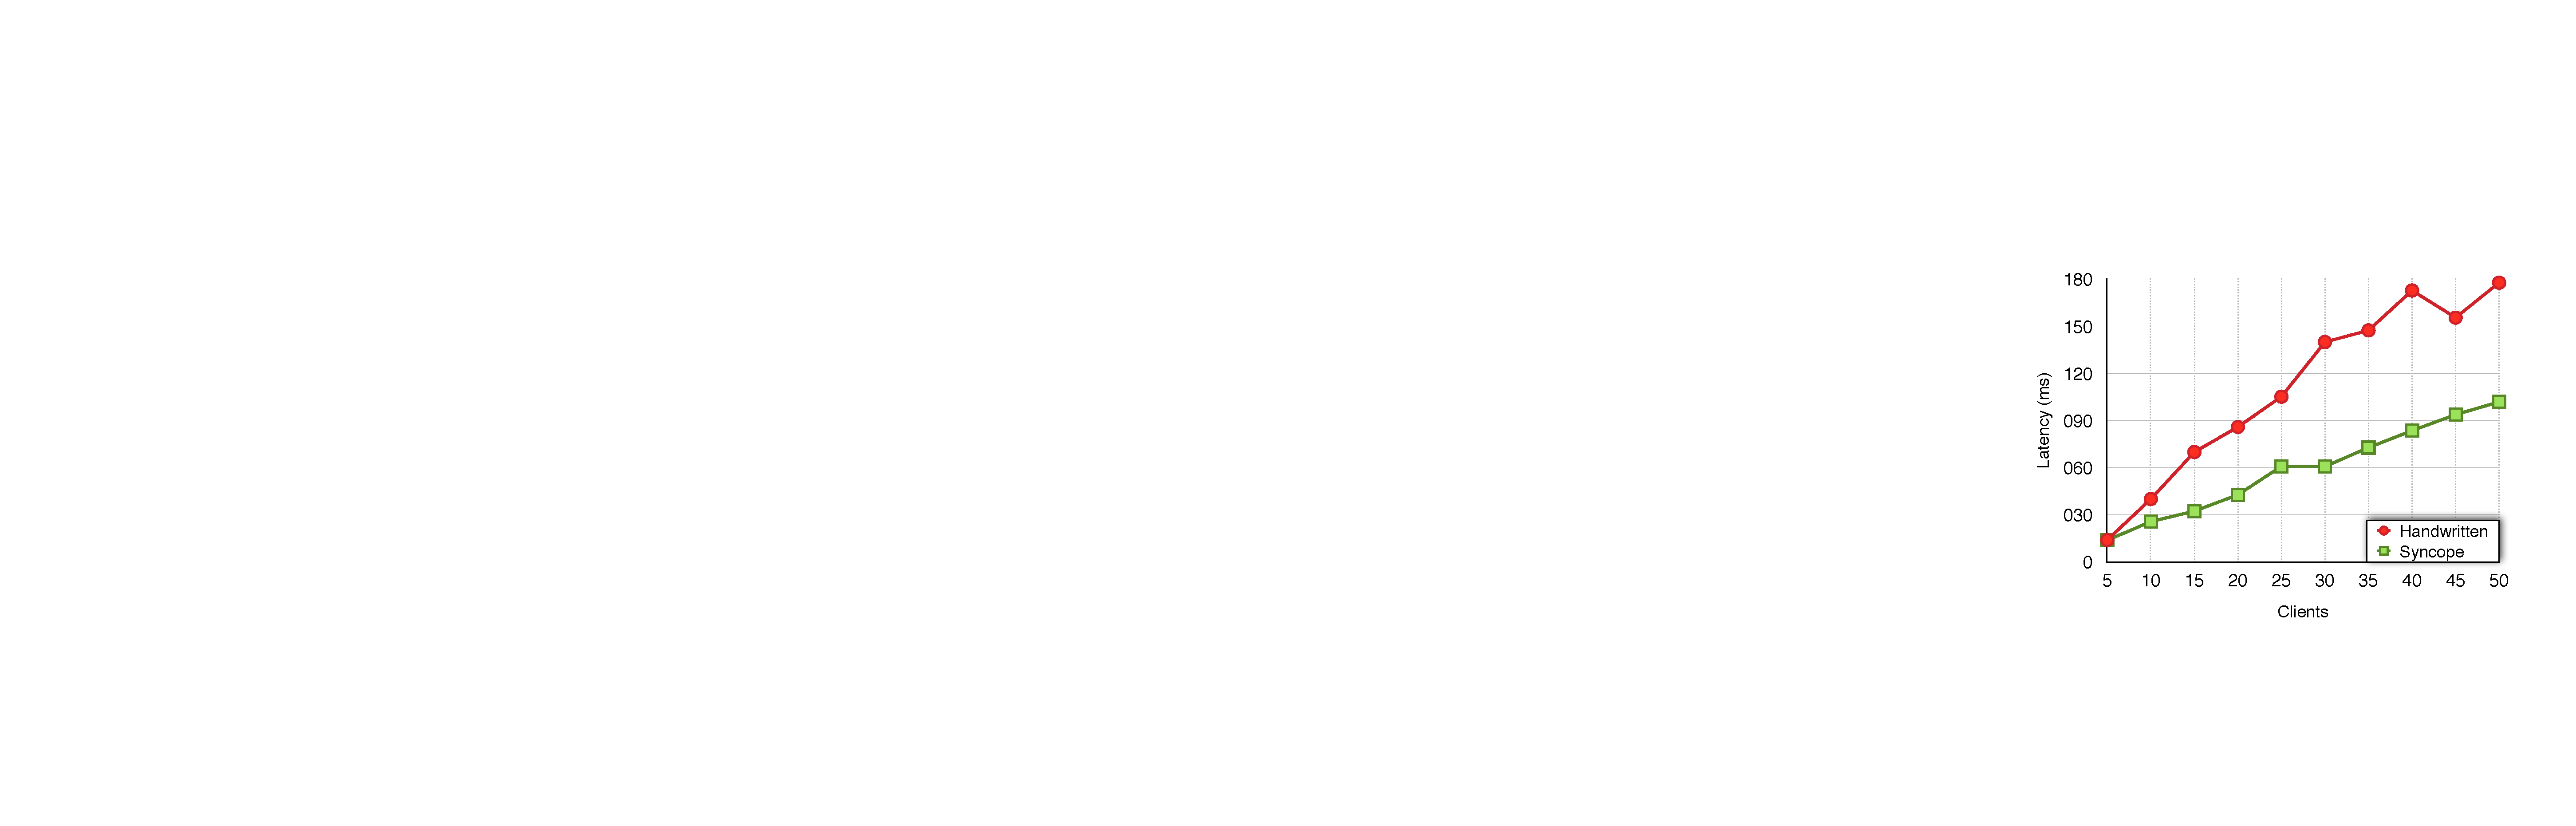
\includegraphics[scale=0.22]{Figures/comparison.pdf}
	\subcaption*{ \hspace{8mm} (c) Manual RMW}
	\label{subfig:comment_example}
	\end{subfigure} 
\\ \hrulefill
\caption{A distributed application for comment section
management}
\label{fig:eval}
\end{figure}



% performance evaluation
We have deployed \tool on a cloud cluster,
consisting of three fully replicated Cassandra replicas, running on
seperate machines within the same
datacenter. 
Each machine is instantiated with a
\tool shim layer, that responds to clients,  
 which are instantiated on a VM 
co-located with one of the replicas on a machine.
We deploy the cluster on three \texttt{m4.4xlarge} Amazon EC2 instances
in the US-West (Oregon) region, with an inter-machine communication time of 5ms.

% The problem with Cassandra
%%%SJ: is there any references you can cite to indicate this
%%%decision is realistic, or consistent with other papers in this space?
Inter-replica communication in Cassandra uses TCP connections, causing
all messages to get delivered with no loss and reordering, which is in
practice, far more consistent than EC, and masks out the performance
gain from our fine-grained consistency guarantees.  Consequently, to
simulate a realistic EC environment, we injected artificial message
losses in \tool's shim layer, forcing random messages to be delayed
for 1s, simulating messages losses in a network with 600ms RTT
(observed inter-replica RTT value during our experiments is 600ms).

% The problem with Cassandra
% ! 
% !
% PLEASE ADD CITATIONS/EDIT -- I WILL BE LOOKING FOR CITATIONS

%The latency and staleness gain using fine-grained consistency
Fig.~\ref{fig:eval}(a) and \ref{fig:eval}(b) represent
our experimental results, with a workload generated 
by 50 concurrent clients repeatedly running sessions, each composed of three
operations, where operations uniformly choose from 5 objects,
performed under a specified consistency level. 
We increase the
percentage of delayed messages from 0 to 14.  Each experiment ran for
100 repeaded sessions per client. In addition to client perceived
latency, we also measure the staleness of operations, which we define as
the average ratio of the number of visible effects,
to the number of all available effects, when executing an operation.

% latency result
In the first set of experiments, we measure latency under
three different \LB{} contracts, all implemented in \tool. As
expected,
causal consistency and RMW experience respectively the highest and the
lowest
performance loss as the percentage of lost messages is increased\footnote{In fact, 
they define the strongest and the weakest
\LB{} dependency relations expressable in our language:
$(\xrightarrow{\soZ})$ and $(\xrightarrow{(\soZ\cup\visZ)^*})$}.
With only a 4\% percent message loss rate, we see $17\%$ higher latency under an MR
contract compared to RMW, and similarly 67\% higher latency in CC
compared to MR; with $10$ percent message loss, the numbers are
increased to $18\%$ and $87\%$.


%latency result
Similarly, we repeated the experiment with 3 \UB{} contracts. Here, a
\emph{causal visibility} (CV) contract (i.e. {\footnotesize $ \forall a.
a\xrightarrow{(\soZ\cup\visZ)^*;\visZ}\hat{\eta}\Rightarrow a\xrightarrow{\visZ}
\hat{\eta} $}), yields the most stale data when the percentage of lost
messages is increased, whereas staleness in MW is the lowest and is
barely effected. We report $3\%$ ($6\%$) difference 
between staleness of data under MW and 2VIS, and $4\%$ ($7\%$)
difference between 2VIS and CV,
at four (ten) percante message
loss rate.



%handwritten compared
Finally, in order to provide evidence on the practicality of \tool, we
implemented an ad-hoc mechanism to prevent the lost-updates anomaly,
for a simple counter application. Fig.~\ref{fig:eval}(c) shows the
latency results of this application compared to the same in \tool,
under the same setting as before (albeit with no message loss).  We
see $78\%$ higher latency for the handwritten code compared to \tool
with 50 concurrent clients. The reason hand-written code performs
worse than \tool is because it relies on certain cassandra-specific
features that are not optimized for the current purpose (each time a
new session is created, it performs a strongly-consistent schema
alteration to create a new column that records the sequence number of
the last update from that session to every object).  Short of
replicating the \tool's shim layer-based approach, we found no other
way to enforce the required consistency guarantee beyond the one we
implemented. Beyond the performance numbers, the ad hoc approach to
consistency enforcement is also qualitatively inferior since it
required significant re-engineering of the counter application (nearly
40\% of the code needed refractoring to perform book-keeping needed
for the ad hoc approach to work). With \tool, however, no refractoring
was needed to enforce the required consistency.










































